\begin{frame}{Automatic Temperature Tuning}
\begin{itemize}
    \item Choosing the optimal temperature is non-trivial (tuned for each task)
    \item Constrained optimization problem:
\end{itemize}
\[
\max \sum_{t} \mathbb{E}_{(\mathbf{s}_t, \mathbf{a}_t) \sim \rho_\pi}\!\left[ r(\mathbf{s}_t, \mathbf{a}_t) + \alpha \mathcal{H}(\pi(\,\cdot \mid \mathbf{s}_t)) \right]
\]
\[
\max_{\pi_{0:T}} \mathbb{E}_{\rho_\pi}\!\left[ \sum_{t=0}^{T} r(\mathbf{s}_t, \mathbf{a}_t) \right] \;\; \text{s.t.}\;\; \mathbb{E}_{(\mathbf{s}_t, \mathbf{a}_t) \sim \rho_\pi}\!\left[ -\log(\pi_t(\mathbf{a}_t \mid \mathbf{s}_t)) \right] \geq \mathcal{H}\;\; \forall t
\]
\end{frame}
\begin{frame}{Dual Problem for the Constrained Optimization}
\textbf{Unroll the expectation}
\[
\max_{\pi_0}\!\left( \mathbb{E}[r(\mathbf{s}_0, \mathbf{a}_0)] + \max_{\pi_1}\!\left( \mathbb{E}[\ldots] + \boxed{\max_{\pi_T} \mathbb{E}[r(\mathbf{s}_T, \mathbf{a}_T)]} \right) \right)
\]

\textbf{For the last time step in the trajectory}
\begin{align*}
\max_{\pi_T} \mathbb{E}_{(\mathbf{s}_t, \mathbf{a}_t) \sim \rho_\pi}\!\left[ r(\mathbf{s}_T, \mathbf{a}_T) \right] &= \min_{\alpha_T \geq 0} \max_{\pi_T} \mathbb{E}\!\left[ r(\mathbf{s}_T, \mathbf{a}_T) - \alpha_T \log \pi(\mathbf{a}_T \mid \mathbf{s}_T) \right] - \alpha_T \mathcal{H}. \\
\arg\min_{\alpha_T} \mathbb{E}_{\mathbf{s}_t, \mathbf{a}_t \sim \pi_t^{*}}\!\left[ -\alpha_T \log \pi_T^{*}(\mathbf{a}_T \mid \mathbf{s}_T; \alpha_T) - \alpha_T \mathcal{H} \right]. & \\
\end{align*}
\end{frame}
\begin{frame}{Dual Problem for the Constrained Optimization}
\textbf{Similarly, for the previous time step}
\begin{align*}
\max_{\pi_{T-1}}\!\Big( \mathbb{E}[r(\mathbf{s}_{T-1}, \mathbf{a}_{T-1})] &+ \max_{\pi_T} \mathbb{E}[r(\mathbf{s}_T, \mathbf{a}_T)] \Big) \tag{16} \\
&= \max_{\pi_{T-1}}\!\big( Q_{T-1}^{*}(\mathbf{s}_{T-1}, \mathbf{a}_{T-1}) - \alpha_T \mathcal{H} \big) \\
&= \min_{\alpha_{T-1} \geq 0} \max_{\pi_{T-1}}\!\Big( \mathbb{E}[Q_{T-1}^{*}(\mathbf{s}_{T-1}, \mathbf{a}_{T-1})] - \mathbb{E}[\alpha_{T-1} \log \pi(\mathbf{a}_{T-1} \mid \mathbf{s}_{T-1})] - \alpha_{T-1} \mathcal{H} \Big) + \alpha_T^{*} \mathcal{H}.
\end{align*}
\[
\alpha_t^{*} = \arg\min_{\alpha_t} \mathbb{E}_{\mathbf{a}_t \sim \pi_t^{*}}\!\left[ -\alpha_t \log \pi_t^{*}(\mathbf{a}_t \mid \mathbf{s}_t; \alpha_t) - \alpha_t \bar{\mathcal{H}} \right]
\]
\end{frame}
\begin{frame}[plain]
\begin{figure}
    \centering
    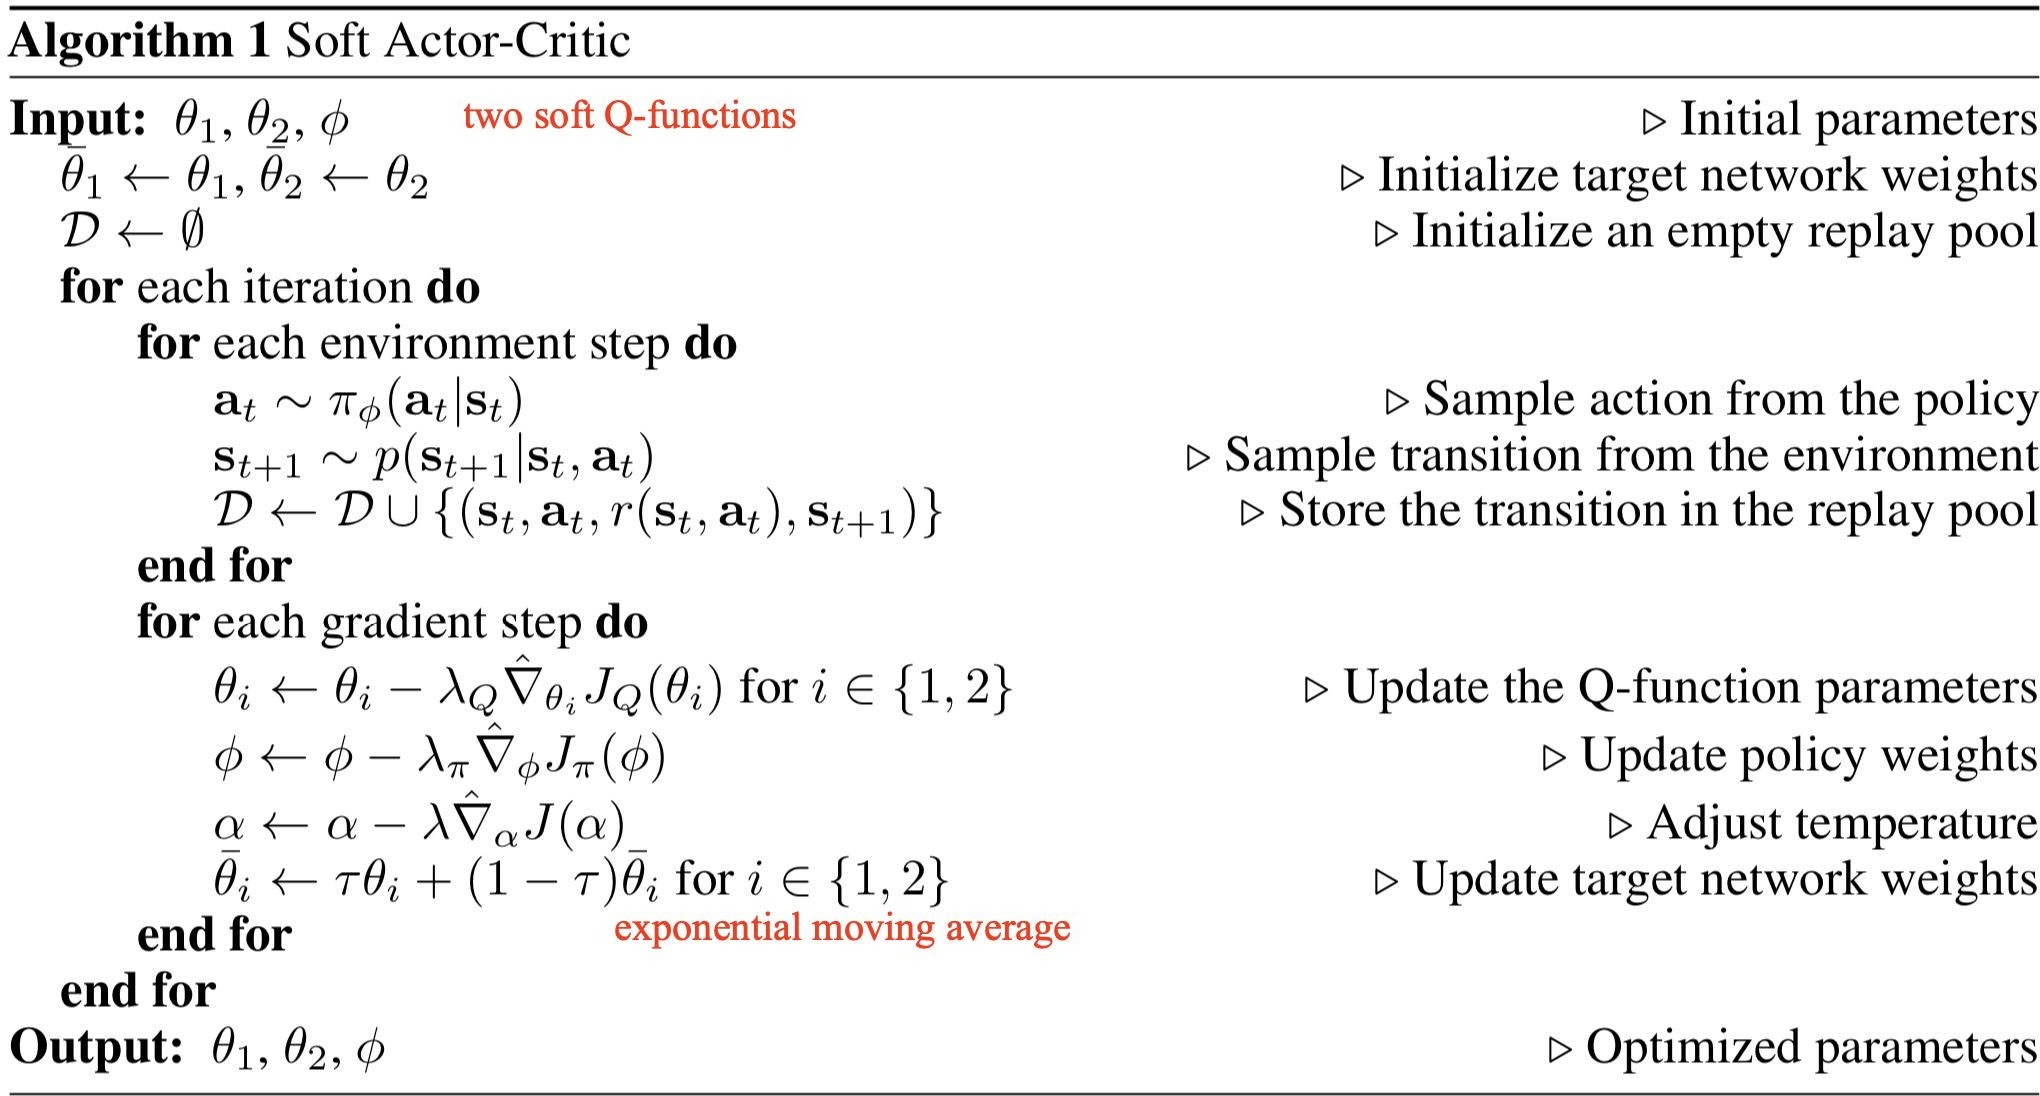
\includegraphics[width=\textwidth,height=0.95\textheight,keepaspectratio]{images/soft-actor-critic/figures/sac-algorithm-paper.jpg}
\end{figure}
\end{frame}
